\subsection{Abertura mínima para chute a gol}

Somente o peso do parâmetro que permite chute a gol foi alterado para $5$.  Os
resultados no planejamento são apresentados na Figura~\ref{fig:min_gap_5}.
Conforme pode ser visto, somente no ambiente de ataque houve uma mudança grande,
gerando uma ação de chute no lugar de uma ação de passe.

\begin{figure}[H]
  \centering
  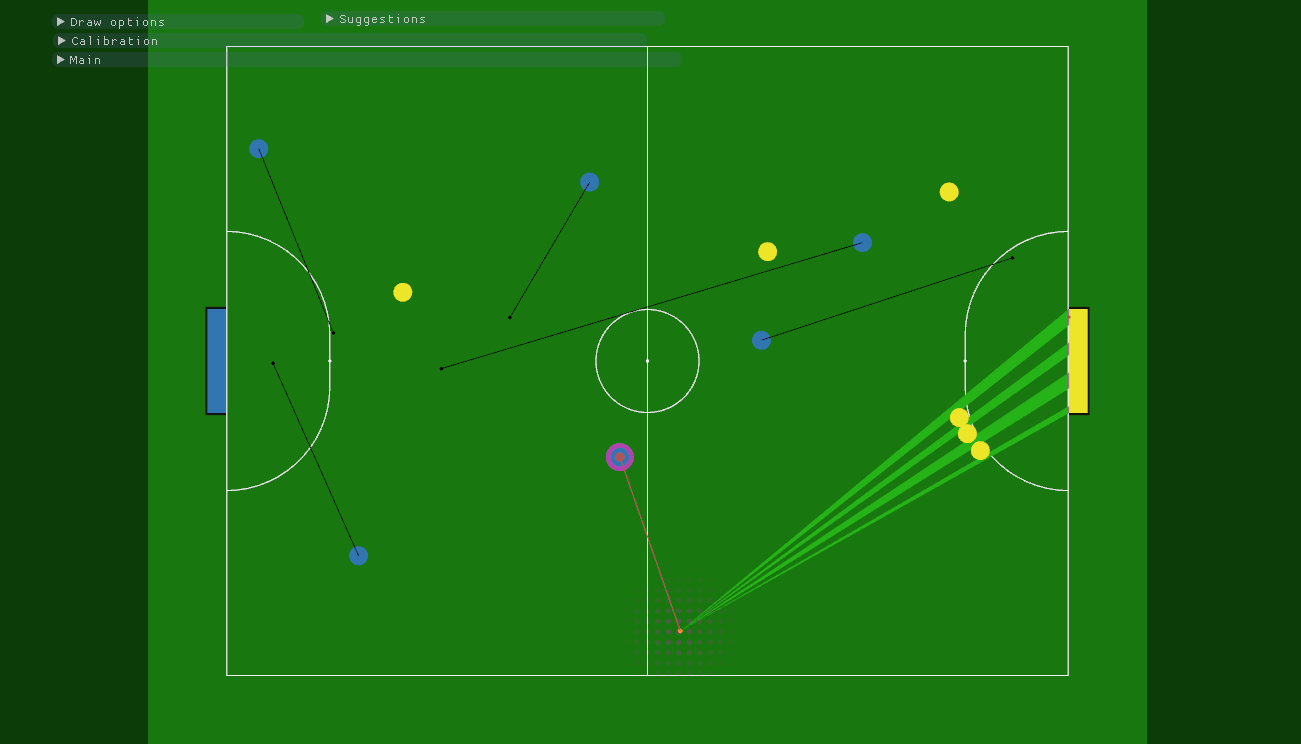
\includegraphics[width= 0.8\linewidth]{result/min_gap_atq_5}
  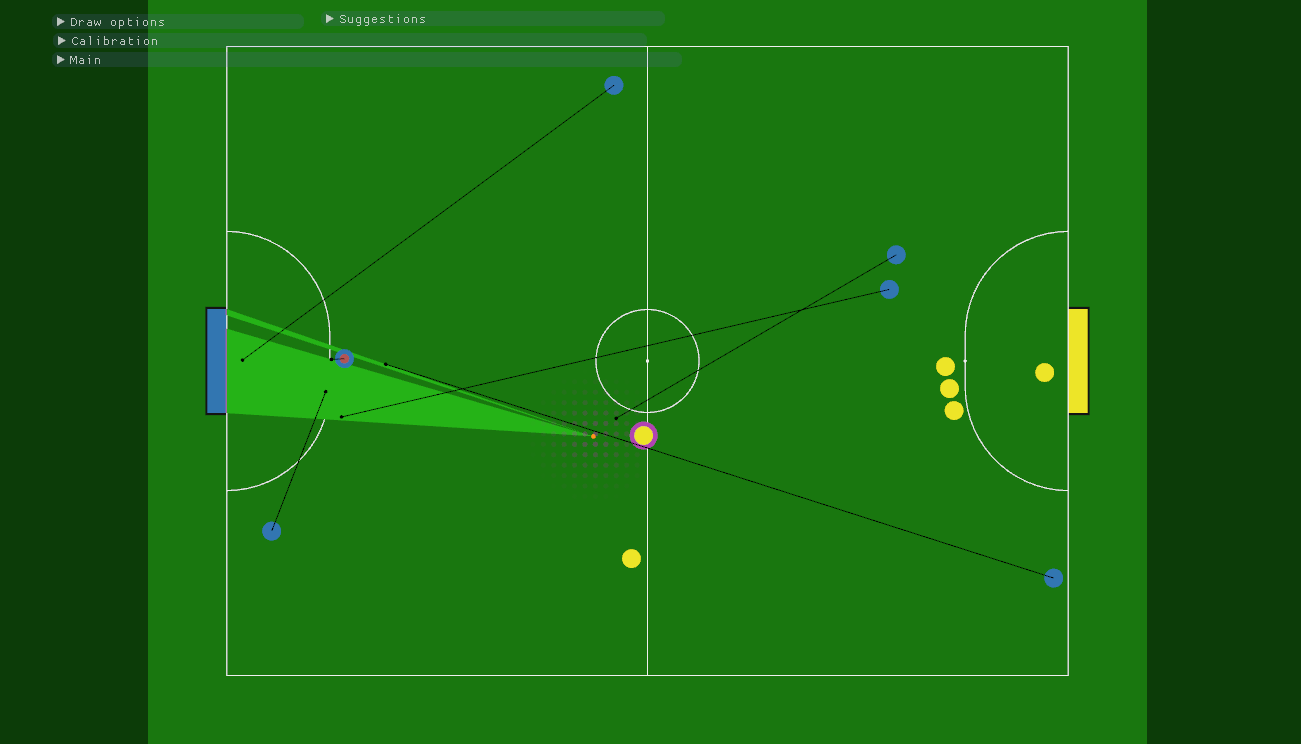
\includegraphics[width= 0.8\linewidth]{result/min_gap_def_5}
  \caption{Planejamento com os parâmetros iniciais e com a abertura mínima para
  chute alterado para $5$.  No ataque (acima) e na defesa (abaixo)}\label{fig:min_gap_5}
\end{figure}

% vim: tw=80 et ts=2 sw=2 sts=2 ft=tex spelllang=pt_br,en
